\documentclass[A5paper 11pt]{article}
%_______________________________________________________________

\usepackage[spanish]{babel}

\usepackage[a5paper,top=1cm,bottom=.9cm,left=3cm,right=2.5cm,marginparwidth=1.75cm]{geometry}

\usepackage{amsmath}

\usepackage{graphicx}

\usepackage[usenames]{xcolor}

\usepackage[utf8]{inputenc}

\usepackage{amssymb}

%_______________________________________________________________
\pagecolor{blue}


\begin{document}
{\centering\huge{{Serie ó Película}\\
Pérez Álvarez Erick Yahel\\
22/sep/2022}\\}


\section{MÁTRIX}

\subsection{\textit{RESEÑA}}
Matrix es una película de acción y ciencia ficción dirigida por las hermanas Lilly y Lana Wachowski estrenada en 1999. Forma parte de una tetralogía conformada por The Matrix (1999), Matrix Reloaded (2003) , Matrix Revolutions (2003) y The Matrix Resurrections (2021).\\
    
Matrix narra la aventura de Neo, un joven hacker que es convocado por el movimiento de resistencia liderado por Morfeo, que lucha contra la dominación de los seres humanos por las máquinas. Morfeo le ofrece dos pastillas de diferentes colores: con una continuará en la ilusión, con la otra descubrirá la verdad.

El protagonista escoge la píldora roja y despierta en una cápsula, de esta manera descubre que la raza humana está dominada por la inteligencia artificial, y vive atrapada en un programa de ordenador y sirve solo como una fuente de energía. Neo se da cuenta de que la resistencia cree que él es el Elegido, un mesías que liberará a la humanidad de la esclavitud de Matrix.

Aunque dude de su destino a lo largo de todo el camino, aprende a superar las reglas de simulación. Consigue salvar a Morfeo, que había sido secuestrado, y derrota al agente Smith tras un duelo en el que demuestra su valía como guerrero y confirma que es el Elegido.
\newpage
\subsection{\textit{ELENCO Y PRODUCTORES}}
  \begin{itemize}
    \item[1.-]Keanu Reeves (Personaje principal)
    \item[2.-]Laurance Fishburne (Personaje principal)
    \item[3.-]Carrie-Anne Moss (Personaje principal)
    \item[4.-]Hugo Weaving (Personaje principal)
    \item[5.-]Gloria Foster (Personaje terciario)
    \item[6.-]Joe Pantoliano (Personaje terciario)
    \item[7.-]Hermanas Wachowski (dirección)
    \item[8.-]Joel Silver (producción)
    \item[9.-]Lilly Wachowski · Lana Wachowski (guión)
    \item[10.-]Don Davis (música)
    \item[11.-]Bill Pope (fotografía)
    \item[12.-]Zach Staenberg (montaje)
  \end{itemize}
  
\newpage

\subsection{\textit{PERSONAJES}}
\begin{itemize}
    \item[$\delta$]\fcolorbox{black}{red}{Neo} \textit{Informático durante el día, Thomas A. Anderson esconde un secreto: de noche trabaja como hacker utilizando el nombre de Neo. Es localizado por Morfeo y Trinity y descubre la verdad sobre Matrix, convirtiéndose en el Elegido que salvará a la humanidad de la esclavitud.}
    \item[$\delta$]\fcolorbox{black}{yellow}{Morpheo} \textit{Morfeo es el líder de la lucha humana contra la dominación de las máquinas. Por haber "despertado" hace muchos años, conoce los trucos de la simulación y está seguro de que encontrará al Elegido. Como un verdadero maestro, guía a Neo a lo largo de toda la narración.}
    \item[$\delta$]\fcolorbox{black}{white}{Trinity}\textit{Trinity es una famosa hacker que va en busca de Neo a través de Matrix. Aunque los agentes la subestiman porque creen que es débil, Trinity logra escapar de ellos y derrotarlos en varias ocasiones. Acompaña a Neo en la misión de salvar a Morfeo, arriesgando su propia vida. Su fé y el amor inquebrantable hacia el protagonista es lo que le hacen resistir hasta el final.}
    \item[$\delta$]\fcolorbox{black}{pink}{Agente Smith}\textit{El agente Smith representa a la autoridad en Matrix, su responsabilidad es mantener el orden y neutralizar la actuación de la resistencia. Puesto que forma parte de un programa de ordenador, posee facultades que lo convierten en un enemigo casi imposible de derrotar. Pese a que no es humano, manifiesta emociones como la rabia y la desesperación.}
     
\end{itemize}
  
\newpage
%   

   \begin{figure}
     \raggedleft 
     \caption{escena matrix} 
     %NO PUDE QUITARLE LA NUMERACION :(
 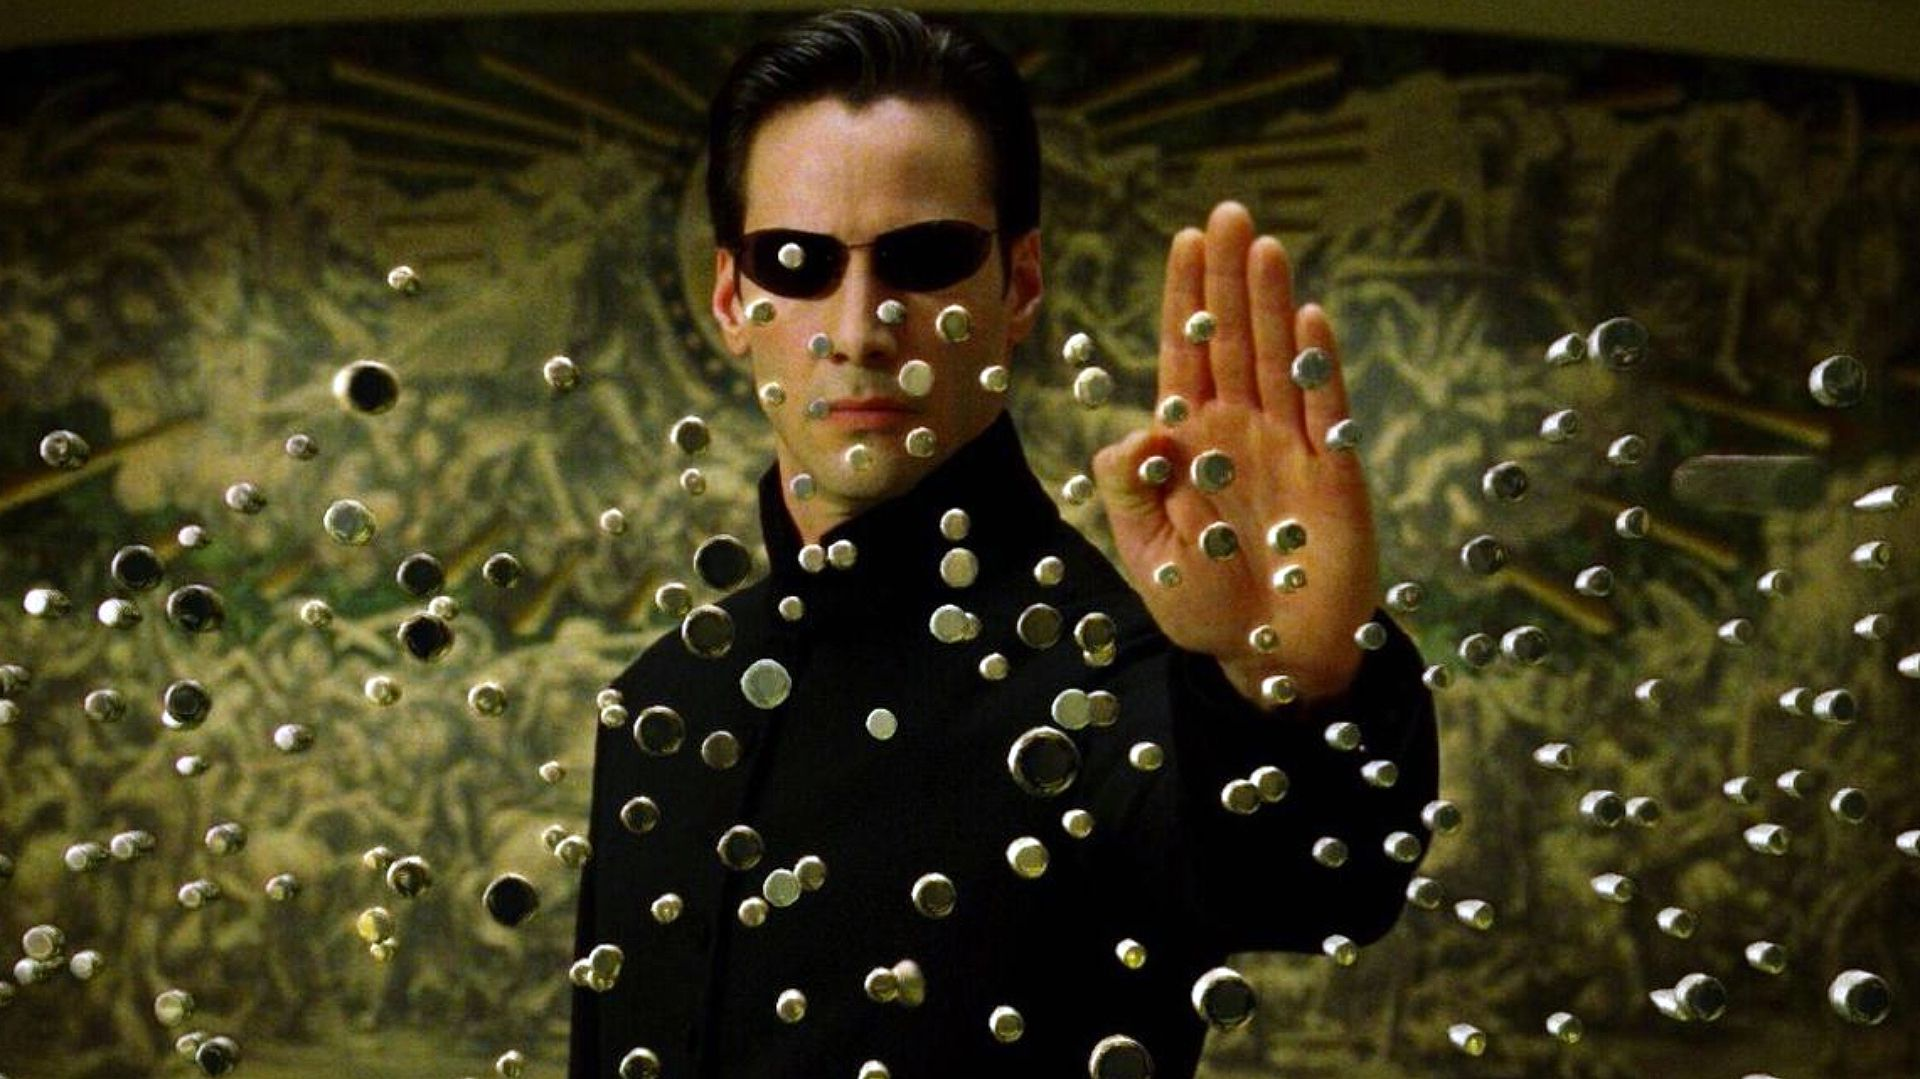
\includegraphics[scale=0.1, angle=15]{matrix.jpg}
 
     \end{figure}



\section{\textit{¿POR QUÉ ME GUSTÓ?}}

\textcolor{green}{Me gustan las peliculas distopicas con historias de robots etc}\textcolor{yellow}{, y en general la historia contiene muchas referencias filosoficas y con un trasfondo muy profundo, las cuales me agradan mucho}\textcolor{cyan}{, aparte, despues de ver la pelicula te quedas con ganas de saber que paso con la humanidad y por que llegaron a esa situacion :o} \\
\newpage
\begin{figure}
    \centering
    
\includegraphics[scale=0.1, angle=-18]{keanu.jpg}
    \caption{keanu es dios, que puedo decir}
\end{figure}

\begin{figure}
    \centering
    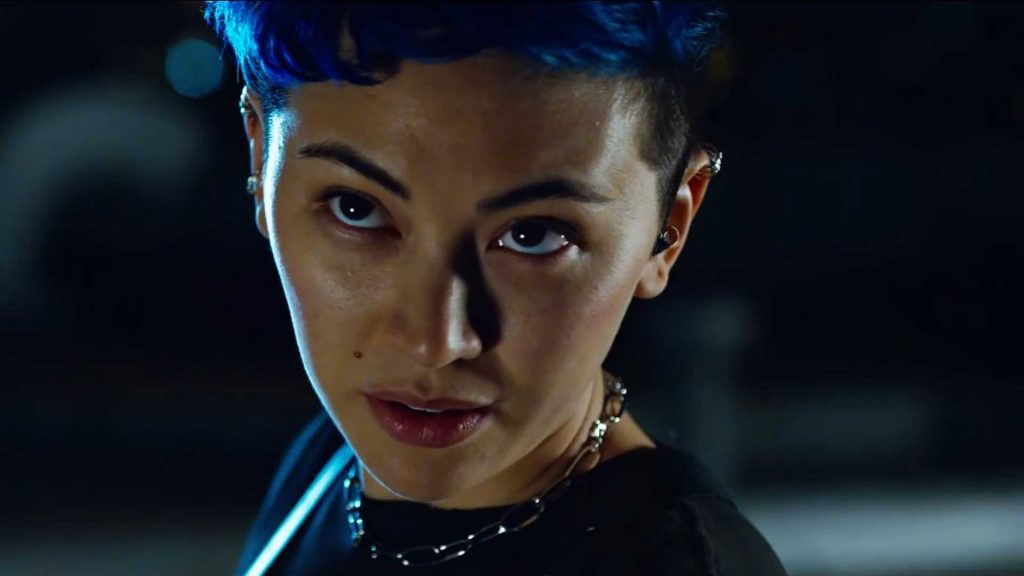
\includegraphics[scale=0.2, angle=8]{R.jpg}
    \caption{no me agrado, tuvo un desarrollo de personaje muy pobre}
\end{figure}

\end{document}